%--- ausblick

\section{Ausblick - Problem des Handlungsreisenden (TSP)}

Mithilfe der aufgearbeiteten Inhalte soll das Problem des Handlungsreisenden (\textit{engl.} \enquote{travelling salesman problem}) bearbeitet werden.\\
Dabei handelt es sich um einen Handlungseisenden, der bei einer Stadt startet und weitere Städte in einem Rundgang jeweils nur einmal besuchen möchte.
Somit dürfen keine Städte doppelt besucht werden, es darf aber auch keine Stadt aus der Rundreise ausgelassen werden.
Die Stadt, in welcher der Handlungsreisende seine Reise beginnt, ist gleichzeitig die letzte Stadt der Rundreise.

Hierbei handelt es sich um ein kombinatorisches Problem analog der Methodik \enquote{Ziehen ohne Zurücklegen mit Reihenfolge}.\\
Möchte der Handlungsreisende neben seiner Start-/Zielstadt beispielsweise 20 weitere Städte ansiedeln, so gibt es $20! = 2,433*10^18$ Möglichkeiten, die Rundreise zu bewältigen. Alle Möglichkeiten anhand eines Brute-Force-Algorithmus einzeln auszuprobieren und anschließend den optimalen kürzesten Weg zu wählen, ist bei dieser Eingabelänge schon nicht mehr realistisch.

Abbildung \ref{fig:tsp} zeigt eine von vielen Möglichkeiten der Rundreise beispielhaft an und illustriert die kombinatorische Komplexität des Problems.

\begin{figure}[H]
\centering
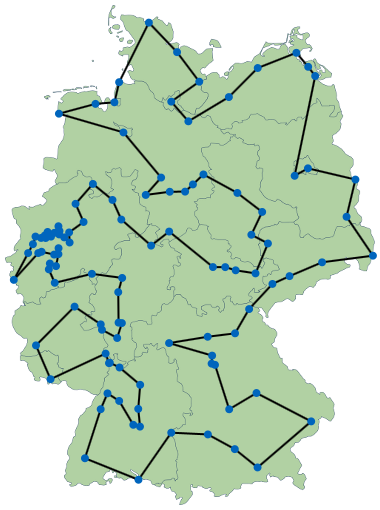
\includegraphics[width=0.75\textwidth]{img/tsp.png}
\caption{Problem des Handlungsreisenden}
\label{fig:tsp}
\end{figure}

Für die Durchführung unterschiedlicher Genetischer Algorithmen werden die Chromosome anhand der Indizes der einzelnen Städte codiert.
Insofern wird der Fokus auf die Crossover-Strategien und das Experimentieren mit den Parameterkonfigurationen gelegt werden, um das Problem des Handlungsreisenden zu bearbeiten. Abschließend sollen die unterschiedlichen Strategien miteinander verglichen werden.
